\documentclass{amsart}
\usepackage{tikz}
\usepackage{amsmath, amssymb, amsthm} 
\usepackage{hyperref} 
\usepackage{geometry} 
\usepackage{xcolor}
\geometry{margin=1in} 

\definecolor{codegreen}{rgb}{0,0.6,0}
\definecolor{codegray}{rgb}{0.5,0.5,0.5}
\definecolor{codepurple}{rgb}{0.58,0,0.82} 
\definecolor{backcolour}{rgb}{0.95,0.95,0.92}
\definecolor{maingreen}{HTML}{7EBE91}

\theoremstyle{plain}
\newtheorem{theorem}{Theorem}[section]
\newtheorem{lemma}[theorem]{Lemma}

\theoremstyle{definition}
\newtheorem{definition}[theorem]{Definition}

\theoremstyle{remark}
\newtheorem{remark}[theorem]{Remark}

\title{PhD Project Proposal: Title TBD}
\author{Matthew Knowles}
\date{\today}

\begin{document}

\maketitle

\section{Backgound}
While clinical trials are the gold standard experiment for assessing the efficacy and safety of a novel treatment, the limited financial and operational resources of clinical trial sponsors means that most trials only compare the new, experimental treatment against the standard of care for the given indication. This presents a fundamental issue for decision makers (such as the National Institute for Health and Clinical Excellence (NICE)) as there is often no direct evidence comparing two novel treatments.\\

Indirect Treatment Comparisons (ITCs) present decision makers with a method for synthesising evidence from multiple trials into a coherent assessment of the treatment landscape for a given indication. Several methods exist for performing such assessments.W

\begin{figure}[h]
    \centering
    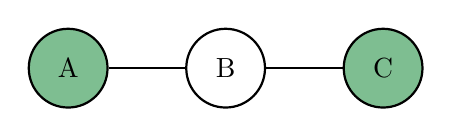
\begin{tikzpicture}[node distance=2cm, thick, main/.style={circle, draw, minimum size=1cm}]
        \node[main, fill = maingreen] (A) {A};
        \node[main] (B) [right of=A] {B};
        \node[main, fill = maingreen] (C) [right of=B] {C};
        \draw (A) -- (B);
        \draw (B) -- (C);
    \end{tikzpicture}
    \caption{A simple network of trials}
    \label{fig:simpleNetwork}
\end{figure}



\end{document}
